
%{{第六十回}}{第六十回}}

\chapter{茉莉粉替去蔷薇硝\\玫瑰露引来茯苓霜}

{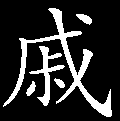
\includegraphics[width=3mm]{../Images/00005}前回叙蔷薇硝,嘎然便住,至此回方结过蔷薇案。接笔转出玫瑰露,引起茯苓霜,又嘎然便住。着笔如苍鹰搏兔,青狮戏球,不肯下一死爪。绝世妙文!}

话说袭人因问平儿,何事这等忙乱。平儿笑道:``都是世人想不到的,说来也好笑,等几日告诉你,如今没头绪呢,且也不得闲儿。''一语未了,只见李纨的丫鬟来了,说:``平姐姐可在这里,奶奶等你,你怎么不去了?''平儿忙转身出来,口内笑说:``来了,来了。''袭人等笑道:``他奶奶病了,他又成了香饽饽了,都抢不到手。''平儿去了不提。

这里宝玉便叫春燕:``你跟了你妈去,到宝姑娘房里给莺儿几句好话听听,也不可白得罪了他。''春燕答应了,和他妈出去。宝玉又隔窗说道:``不可当着宝姑娘说,仔细反叫莺儿受教导。''

娘儿两个应了出来,一壁走着,一面说闲话儿。春燕因向他娘道:``我素日劝你老人家再不信,何苦闹出没趣来才罢。''他娘笑道:``小蹄子,你走罢,俗语道:`不经一事,不长一智。'我如今知道了。你又该来支问着我。''春燕笑道:``妈,你若安分守己,在这屋里长久了,自有许多的好处。我且告诉你句话:宝玉常说,将来这屋里的人,无论家里外头的,一应我们这些人,他都要回太太全放出去,与本人父母自便呢。{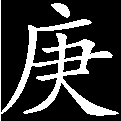
\includegraphics[width=3mm]{../Images/00004}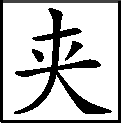
\includegraphics[width=3mm]{../Images/00012}\footnotesize \kaishu 补前文不足处。}你只说这一件可好不好?''他娘听说,喜的忙问:``这话果真?''春燕道:``谁可扯这谎做什么?''婆子听了,便念佛不绝。

当下来至蘅芜苑中,正值宝钗、黛玉、薛姨妈等吃饭。莺儿自去泡茶,春燕便和他妈一径到莺儿前,陪笑说``方才言语冒撞了,姑娘莫嗔莫怪,特来陪罪''等语。莺儿忙笑让坐,又倒茶。他娘儿两个说有事,便作辞回来。忽见蕊官赶出叫:``妈妈、姐姐,略站一站。''一面走上来,递了一个纸包与他们,说是蔷薇硝,带与芳官去擦脸。春燕笑道:``你们也太小气了,还怕那里没这个与他,巴巴的你又弄一包给他去。''蕊官道:``他是他的,我送的是我的。好姐姐,千万带回去罢。''春燕只得接了。娘儿两个回来,正值贾环贾琮二人来问候宝玉,也才进去。春燕便向他娘说:``只我进去罢,你老不用去。''他娘听了,自此便百依百随的,不敢倔强了。

春燕进来,宝玉知道回复,便先点头。春燕知意,便不再说一语,略站了一站,便转身出来,使眼色与芳官。芳官出来,春燕方悄悄的说与他蕊官之事,并与了他硝。宝玉并无与琮环可谈之语,因笑问芳官手里是什么。芳官便忙递与宝玉瞧,又说是擦春癣的蔷薇硝。宝玉笑道:``亏他想得到。''贾环听了,便伸着头瞧了一瞧,又闻得一股清香,便弯着腰向靴桶内掏出一张纸来托着,笑说:``好哥哥,给我一半儿。''宝玉只得要与他。芳官心中因是蕊官之赠,不肯与别人,连忙拦住,笑说道:``别动这个,我另拿些来。''宝玉会意,忙笑包上,说道:``快取来。''

芳官接了这个,自去收好,便从奁中去寻自己常使的。启奁看时,盒内已空,心中疑惑,早间还剩了些,如何没了?因问人时,都说不知。麝月便说:``这会子且忙着问这个,不过是这屋里人一时短了。你不管拿些什么给他们,他们那里看得出来?快打发他们去了,咱们好吃饭。''芳官听了,便将些茉莉粉包了一包拿来。贾环见了就伸手来接。芳官便忙向炕上一掷。贾环只得向炕上拾了,揣在怀内,方作辞而去。

原来贾政不在家,且王夫人等又不在家,贾环连日也便装病逃学。如今得了硝,兴兴头头来找彩云。正值彩云和赵姨娘闲谈,贾环嘻嘻向彩云道:``我也得了一包好的,送你擦脸。你常说,蔷薇硝擦癣,比外头的银硝强。你且看看,可是这个?''彩云打开一看,``嗤''的一声笑了,说道:``你是和谁要来的?''贾环便将方才之事说了。彩云笑道:``这是他们哄你这乡老呢。这不是硝,这是茉莉粉。''贾环看了一看,果然比先的带些红色,闻闻也是喷香,因笑道:``这也是好的,硝粉一样,留着擦罢,自是比外头买的高便好。''彩云只得收了。赵姨娘便说:``有好的给你!谁叫你要去了,怎怨他们耍你!依我,拿了去照脸摔给他去,趁着这回子撞尸的撞尸去了,挺床的便挺床,吵一出子,大家别心净,也算是报仇。莫不是两个月之后,还找出这个碴儿来问你不成?便问你,你也有话说。宝玉是哥哥,不敢冲撞他罢了。难道他屋里的猫儿狗儿,也不敢去问问不成!''贾环听说,便低了头。彩云忙说:``这又何苦生事,不管怎样,忍耐些罢了。''赵姨娘道:``你快休管,横竖与你无干。乘着抓住了理,骂给那些浪淫妇们一顿也是好的。''又指贾环道:``呸!你这下流没刚性的,也只好受这些毛崽子的气!平白我说你一句儿,或无心中错拿了一件东西给你,你倒会扭头暴筋瞪着眼蹾摔娘。这会子被那起屄崽子耍弄也罢了。你明儿还想这些家里人怕你呢。你没有屄本事,我也替你羞。''贾环听了,不免又愧又急,又不敢去,只摔手说道:``你这么会说,你又不敢去,指使了我去闹。倘或往学里告去捱了打,你敢自不疼呢?遭遭儿调唆了我闹去,闹出了事来,我捱了打骂,你一般也低了头。这会子又调唆我和毛丫头们去闹。你不怕三姐姐,你敢去,我就伏你。''只这一句话,便戳了他娘的肺,便喊说:``我肠子爬出来的,我再怕不成!这屋里越发有的说了。''一面说,一面拿了那包子,便飞也似往园中去。彩云死劝不住,只得躲入别房。贾环便也躲出仪门,自去顽耍。

赵姨娘直进园子,正是一头火,顶头正遇见藕官的干娘夏婆子走来。见赵姨娘气恨恨的走来,因问:``姨奶奶那去?''赵姨娘又说:``你瞧瞧,这屋里连三日两日进来的唱戏的小粉头们,都三般两样掂人分两放小菜碟儿了。若是别一个,我还不恼,若叫这些小娼妇捉弄了,还成个什么!''夏婆子听了,正中己怀,忙问因何。赵姨娘悉将芳官以粉作硝轻侮贾环之事说了。夏婆子道:``我的奶奶,你今日才知道,这算什么事。连昨日这个地方他们私自烧纸钱,宝玉还拦到头里。人家还没拿进个什么儿来,就说使不得,不干不净的忌讳。这烧纸倒不忌讳?你老想一想,这屋里除了太太,谁还大似你?你老自己撑不起来;但凡撑起来的,谁还不怕你老人家?如今我想,乘着这几个小粉头儿恰不是正头货,得罪了他们也有限的,快把这两件事抓着理扎个筏子,我在旁作证据,你老把威风抖一抖,以后也好争别的礼。便是奶奶姑娘们,也不好为那起小粉头子说你老的。''赵姨娘听了这话,益发有理,便说:``烧纸的事不知道,你却细细的告诉我。''夏婆子便将前事一一的说了,又说:``你只管说去。倘或闹起,还有我们帮着你呢。''赵姨娘听了越发得了意,仗着胆子便一径到了怡红院中。

可巧宝玉听见黛玉在那里,便往那里去了。芳官正与袭人等吃饭,见赵姨娘来了,便都起身笑让:``姨奶奶吃饭,有什么事这么忙?''赵姨娘也不答话,走上来便将粉照着芳官脸上撒来,指着芳官骂道:``小淫妇!你是我银子钱买来学戏的,不过娼妇粉头之流!我家里下三等奴才也比你高贵些的,你都会看人下菜碟儿。宝玉要给东西,你拦在头里,莫不是要了你的了?拿这个哄他,你只当他不认得呢!好不好,他们是手足,都是一样的主子,那里有你小看他的!''芳官那里禁得住这话,一行哭,一行说:``没了硝我才把这个给他的。若说没了,又恐他不信,难道这不是好的?我便学戏,也没往外头去唱。我一个女孩儿家,知道什么是粉头面头的!姨奶奶犯不着来骂我,我又不是姨奶奶家买的。`梅香拜把子------都是奴几'呢!''袭人忙拉他说:``休胡说!''赵姨娘气的便上来打了两个耳刮子。袭人等忙上来拉劝,说:``姨奶奶别和他小孩子一般见识,等我们说他。''芳官捱了两下打,那里肯依,便拾头打滚,泼哭泼闹起来。口内便说:``你打得起我么?你照照那模样儿再动手!我叫你打了去,我还活着!''便撞在怀里叫他打。众人一面劝,一面拉他。晴雯悄拉袭人说:``别管他们,让他们闹去,看怎么开交!如今乱为王了,什么你也来打,我也来打,都这样起来还了得呢!''

外面跟着赵姨娘来的一干的人听见如此,心中各各称愿,都念佛说:``也有今日!''又有那一干怀怨的老婆子见打了芳官,也都称愿。

当下藕官蕊官等正在一处作耍,湘云的大花面葵官,宝琴的荳官,两个闻了此信,慌忙找着他两个说:``芳官被人欺侮,咱们也没趣,须得大家破着大闹一场,方争过气来。''四人终是小孩子心性,只顾他们情分上义愤,便不顾别的,一齐跑入怡红院中。荳官先便一头,几乎不曾将赵姨娘撞了一跌。那三个也便拥上来,放声大哭,手撕头撞,把个赵姨娘裹住。晴雯等一面笑,一面假意去拉。急的袭人拉起这个,又跑了那个,口内只说:``你们要死!有委曲只好说,这没理的事如何使得!''赵姨娘反没了主意,只好乱骂。蕊官藕官两个一边一个,抱住左右手;葵官荳官前后头顶住。四人只说:``你只打死我们四个就罢!''芳官直挺挺躺在地下,哭得死过去。

正没开交,谁知晴雯早遣春燕回了探春。当下尤氏、李纨、探春三人带着平儿与众媳妇走来,忙忙将四个喝住。问起原故,赵姨娘便气的瞪着眼粗了筋,一五一十说个不清。尤李两个不答言,只喝禁他四人。探春便叹气说:``这是什么大事,姨娘也太肯动气了!我正有一句话要请姨娘商议,怪道丫头说不知在那里,原来在这里生气呢,快同我来。''尤氏李氏都笑说:``姨娘请到厅上来,咱们商量。''

赵姨娘无法,只得同他三人出来,口内犹说长说短。探春便说:``那些小丫头子们原是些顽意儿,喜欢呢,和他说说笑笑;不喜欢便可以不理他。便他不好了,也如同猫儿狗儿抓咬了一下子,可恕就恕,不恕时也该叫了管家媳妇们去说给他去责罚,何苦自己不尊重,大吆小喝失了体统。你瞧周姨娘,怎不见人欺他,他也不寻人去。我劝姨娘且回房去煞煞性儿,别听那些混帐人的调唆,没的惹人笑话,自己呆白给人作粗活。心里有二十分的气,也忍耐这几天,等太太回来自然料理。''一席话说得赵姨娘闭口无言,只得回房去了。

这里探春气的和尤氏李纨说:``这么大年纪,行出来的事总不叫人敬伏。这是什么意思,值得吵一吵,并不留体统,耳朵又软,心里又没有计算。这又是那起没脸面的奴才们的调停,作弄出个呆人替他们出气。''越想越气,因命人查是谁调唆的。媳妇们只得答应着,出来相视而笑,都说是``大海里那里寻针去?''只得将赵姨娘的人并园中唤来盘诘,都说不知道。众人没法,只得回探春:``一时难查,慢慢访查,凡有口舌不妥的,一总来回了责罚。''

探春气渐渐平服方罢。可巧艾官便悄悄的回探春说:``都是夏妈和我们素日不对,每每的造言生事。前儿赖藕官烧纸,幸亏是宝玉叫他烧的,宝玉自己应了,他才没话。今儿我与姑娘送手帕去,看见他和姨奶奶在一处说了半天,嘁嘁喳喳的,见了我才走开了。''探春听了,虽知情弊,亦料定他们皆是一党,本皆淘气异常,便只答应,也不肯据此为实。

谁知夏婆子的外孙女儿蝉姐儿便是探春处当役的,时常与房中丫鬟们买东西呼唤人,众女孩儿都和他好。这日饭后,探春正上厅理事,翠墨在家看屋子,因命蝉姐出去叫小幺儿买糕去。蝉儿便说:``我才扫了个大园子,腰腿生疼的,你叫个别的人去罢。''翠墨笑说:``我又叫谁去?你趁早儿去,我告诉你一句好话,你到后门顺路告诉你老娘防着些儿。''说着,便将艾官告他老娘话告诉了他。蝉姐听了,忙接了钱道:``这个小蹄子也要捉弄人,等我告诉去。''说着,便起身出来。至后门边,只见厨房内此刻手闲之时,都坐在阶砌上说闲话呢,他老娘亦在内。蝉儿便命一个婆子出去买糕。他且一行骂,一行说,将方才之话告诉与夏婆子。夏婆子听了,又气又怕,便欲去找艾官问他,又欲往探春前去诉冤。蝉儿忙拦住说:``你老人家去怎么说呢?这话怎得知道的,可又叨登不好了。说给你老防着就是了,那里忙到这一时儿。''

正说着,忽见芳官走来,扒着院门,笑向厨房中柳家媳妇说道:``柳嫂子,宝二爷说了:晚饭的素菜要一样凉凉的酸酸的东西,只别搁上香油弄腻了。''柳家的笑道:``知道。今儿怎遣你来了告诉这么一句要紧话。你不嫌脏,进来逛逛儿不是?''芳官才进来,忽有一个婆子手里托了一碟糕来。芳官便戏道:``谁买的热糕?我先尝一块儿。''蝉儿一手接了道:``这是人家买的,你们还希罕这个。''柳家的见了,忙笑道:``芳姑娘,你喜吃这个?我这里有才买下给你姐姐吃的,他不曾吃,还收在那里,干干净净没动呢。''说着,便拿了一碟出来,递与芳官,又说:``你等我进去替你炖口好茶来。''一面进去,现通开火炖茶。芳官便拿着那糕,问到蝉儿脸上说:``稀罕吃你那糕,这个不是糕不成?我不过说着顽罢了,你给我磕个头,我也不吃。''说着,便将手内的糕一块一块的掰了,掷着打雀儿顽,口内笑说:``柳嫂子,你别心疼,我回来买二斤给你。''小蝉气的怔怔的,瞅着冷笑道:``雷公老爷也有眼睛,怎不打这作孽的!他还气我呢。我可拿什么比你们,又有人进贡,又有人作干奴才,溜你们好上好儿,帮衬着说句话儿。''众媳妇都说:``姑娘们,罢呀,天天见了就咕唧。''有几个伶透的,见了他们对了口,怕又生事,都拿起脚来各自走开了。当下蝉儿也不敢十分说他,一面咕嘟着去了。

这里柳家的见人散了,忙出来和芳官说:``前儿那话儿说了不曾?''芳官道:``说了。等一二日再提这事。偏那赵不死的又和我闹了一场。前儿那玫瑰露姐姐吃了不曾,他到底可好些?''柳家的道:``可不都吃了。他爱的什么似的,又不好问你再要的。''芳官道:``不值什么,等我再要些来给他就是了。''

原来这柳家的有个女儿,今年才十六岁,虽是厨役之女,却生的人物与平、袭、紫、鸳皆类。因他排行第五,便叫他是五儿。{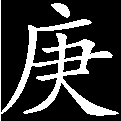
\includegraphics[width=3mm]{../Images/00004}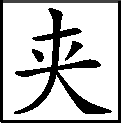
\includegraphics[width=3mm]{../Images/00012}\footnotesize \kaishu 五月之柳,春色可知。}因素有弱疾,故没得差。近因柳家的见宝玉房中的丫鬟差轻人多,且又闻得宝玉将来都要放他们,故如今要送他到那里应名儿。正无头路,可巧这柳家的是梨香院的差役,他最小意殷勤,伏侍得芳官一干人比别的干娘还好。芳官等亦待他们极好,如今便和芳官说了,央芳官去与宝玉说。宝玉虽是依允,只是近日病着,又见事多,尚未说得。

前言少述,且说当下芳官回至怡红院中,回复了宝玉。宝玉正在听见赵姨娘厮吵,心中自是不悦,说又不是,不说又不是,只得等吵完了,打听着探春劝了他去后方从蘅芜苑回来,劝了芳官一阵,方大家安妥。今见他回来,又说还要些玫瑰露与柳五儿吃去,宝玉忙道:``有的,我又不大吃,你都给他去罢。''说着命袭人取了出来,见瓶中亦不多,遂连瓶与了他。

芳官便自携了瓶与他去。正值柳家的带进他女儿来散闷,在那边犄角子上一带地方逛了一回,便回到厨房内,正吃茶歇脚儿。芳官拿了一个五寸来高的小玻璃瓶来,迎亮照看,里面小半瓶胭脂一般的汁子,还道是宝玉吃的西洋葡萄酒。母女两个忙说:``快拿旋子烫滚水,你且坐下。''芳官笑道:``就剩了这些,连瓶子都给你们罢。''五儿听了,方知是玫瑰露,忙接了,谢了又谢。芳官又问他``好些?''五儿道:``今儿精神些,进来逛逛。这后边一带,也没什么意思,不过见些大石头大树和房子后墙,正经好景致也没看见。''芳官道:``你为什么不往前去?''柳家的道:``我没叫他往前去。姑娘们也不认得他,倘有不对眼的人看见了,又是一番口舌。明儿托你携带他有了房头,怕没有人带着逛呢,只怕逛腻了的日子还有呢。''芳官听了,笑道:``怕什么,有我呢。''柳家的忙道:``嗳哟哟,我的姑娘,我们的头皮儿薄,比不得你们。''说着,又倒了茶来。芳官那里吃这茶,只漱了一口就走了。柳家的说道:``我这里占着手,五丫头送送。''

五儿便送出来,因见无人,又拉着芳官说道:``我的话到底说了没有?''芳官笑道:``难道哄你不成?我听见屋里正经还少两个人的窝儿,并没补上。一个是红玉的,琏二奶奶要去还没给人来;一个是坠儿的,也还没补。如今要你一个也不算过分。皆因平儿每每的和袭人说,凡有动人动钱的事,得挨的且挨一日更好。如今三姑娘正要拿人扎筏子呢,连他屋里的事都驳了两三件,如今正要寻我们屋里的事没寻着,何苦来往网里碰去。倘或说些话驳了,那时老了,倒难回转。不如等冷一冷,老太太、太太心闲了,凭是天大的事先和老的一说,没有不成的。''五儿道:``虽如此说,我却性急等不得了。趁如今挑上来了,一则给我妈争口气,也不枉养我一场;{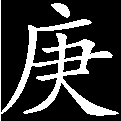
\includegraphics[width=3mm]{../Images/00004}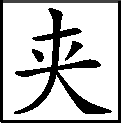
\includegraphics[width=3mm]{../Images/00012}\footnotesize \kaishu 为母。}二则添了月钱,家里又从容些;{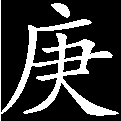
\includegraphics[width=3mm]{../Images/00004}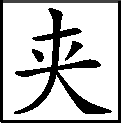
\includegraphics[width=3mm]{../Images/00012}\footnotesize \kaishu 二为家中。}三则我的心开一开,只怕这病就好了。------便是请大夫吃药,也省了家里的钱。''芳官道:``我都知道了,你只放心。''二人别过,芳官自去不提。

单表五儿回来,与他娘深谢芳官之情。他娘因说:``再不承望得了这些东西,虽然是个珍贵物儿,却是吃多了也最动热。竟把这个倒些送个人去,也是个大情。''五儿问:``送谁?''他娘道:``送你舅舅的儿子,昨日热病,也想这些东西吃。如今我倒半盏与他去。''五儿听了,半日没言语,随他妈倒了半盏子去,将剩的连瓶便放在家伙厨内。五儿冷笑道:``依我说,竟不给他也罢了。倘或有人盘问起来,倒又是一场事了。''他娘道:``那里怕起这些来,还了得了。我们辛辛苦苦的,里头赚些东西,也是应当的。难道是贼偷的不成?''说着,一径去了。直至外边他哥哥家中,他侄子正躺着,一见了这个,他哥嫂侄男无不欢喜。现从井上取了凉水,和吃了一碗,心中一畅,头目清凉。剩的半盏,用纸覆着,放在桌上。

可巧又有家中几个小厮,同他侄儿素日相好的,走来问候他的病。内中有一小伙名唤钱槐者,乃系赵姨娘之内侄\href{../Text/part0064_split_000.html\#lnkback_1_a}{\textsuperscript{①}}。他父母现在库上管账,他本身又派跟贾环上学。因他有些钱势,尚未娶亲,素日看上了柳家的五儿标致,和父母说了,欲娶他为妻。也曾央中保媒人再四求告。柳家父母却也情愿,争奈五儿执意不从,虽未明言,却行止中已带出,父母未敢应允。近日又想往园内去,越发将此事丢开,只等三五年后放出来,自向外边择婿了。钱家见他如此,也就罢了。怎奈钱槐不得五儿,心中又气又愧,发恨定要弄取成配,方了此愿。今日也同人来瞧望柳侄,不期柳家的在内。

柳家的忽见一群人来了,内中有钱槐,便推说不得闲,起身便走了。他哥嫂忙说:``姑妈怎么不吃茶就走?倒难为姑妈记挂。''柳家的因笑道:``只怕里面传饭,再闲了出来瞧侄子罢。''他嫂子因向抽屉内取了一个纸包出来,拿在手内送了柳家的出来,至墙角边递与柳家的,又笑道:``这是你哥哥昨儿在门上该班儿,谁知这五日一班,竟偏冷淡,一个外财没发。只有昨儿有粤东的官儿来拜,送了上头两小篓子茯苓霜。馀外给了门上人一篓作门礼,你哥哥分了这些。这地方千年松柏最多,所以单取了这茯苓的精液和了药,不知怎么弄出这怪俊的白霜儿来。说第一用人乳和着,每日早起吃一钟,最补人的;第二用牛奶子;万不得,滚白水也好。我们想着,正宜外甥女儿吃。原是上半日打发小丫头子送了家去的,他说锁着门,连外甥女儿也进去了。本来我要瞧瞧他去,给他带了去的,又想主子们不在家,各处严紧,我又没甚么差使,有要没紧跑些什么。况且这两日风声,闻得里头家反宅乱的,倘或沾带了倒值多的。姑娘来的正好,亲自带去罢。''

柳氏道了生受,作别回来。刚到了角门前,只见一个小幺儿笑道:``你老人家那里去了?里头三次两趟叫人传呢,我们三四个人都找你老去了,还没来。你老人家却从那里来了?这条路又不是家去的路,我倒疑心起来。''那柳家的笑骂道:``好猴儿崽子!\ldots{}\ldots{}''要知端的,且听下回分解。

{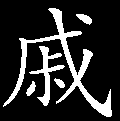
\includegraphics[width=3mm]{../Images/00005}总评:以硝出粉是正笔,以霜陪露是衬笔。前必用茉莉粉,才能构起争端,后不用茯苓霜,亦必败露马脚。须知有此一衬,文势方不径直,方不寂寞。宝光四映,奇彩缤纷。}

% {\href{../Text/part0064_split_000.html\#navto_1_a}{①}``内侄'',除蒙府本改作``内亲'',馀本均同。按赵姨娘之内侄当姓赵。}

